\documentclass{beamer}
\usepackage[utf8]{inputenc}
\usepackage[italian]{babel}
\usepackage{amsmath}
\usepackage{amsfonts}
\usepackage{amssymb}
\usepackage{graphicx}
\usepackage[linesnumbered]{algorithm2e}
\usepackage{float}
\usepackage{mathtools}
\usepackage{subcaption}
\usepackage{wrapfig}
\usepackage{fancyhdr}
\usepackage{xcolor}
\usepackage{hyperref}
\usepackage{listings}

\newcommand{\figcen}[2]{
 \begin{figure}
  \begin{center}
   \includegraphics[width=#1]{#2}
  \end{center}
 \end{figure}
}
\newtheorem{proposition}[theorem]{Proposizione}
\newtheorem{teorema}[theorem]{Teorema}

\definecolor{codeblue}{rgb}{0.21, 0.46, 0.80}
\definecolor{backcolour}{rgb}{0.95,0.95,0.92}
\definecolor{monokai@black}{HTML}{2C2C2A}
\definecolor{monokai@gray}{HTML}{524F52}
\definecolor{monokai@magenta}{HTML}{D33682}
\definecolor{monokai@blue}{HTML}{004C99}

\lstdefinestyle{sql}{
	frame=tb,
	language=SQL,
	backgroundcolor=\color{backcolour},
	aboveskip=3mm,
	belowskip=3mm,
	showstringspaces=false,
	basicstyle={\small\ttfamily},
	breaklines=true,
	breakatwhitespace=true,
	tabsize=1,
	keywordstyle=\color{codeblue},
	stringstyle=\color{monokai@magenta}\ttfamily,
	identifierstyle=\color{monokai@black},
	commentstyle=\color{monokai@blue},
	emphstyle=\color{monokai@red},
	columns=fullflexible
}
\lstdefinestyle{R}{
	frame=tb,
	language=R,
	backgroundcolor=\color{backcolour},
	aboveskip=3mm,
	belowskip=3mm,
	showstringspaces=false,
	basicstyle={\small\ttfamily},
	breaklines=true,
	breakatwhitespace=true,
	tabsize=1,
	keywordstyle=\color{codeblue},
	stringstyle=\color{monokai@magenta}\ttfamily,
	identifierstyle=\color{monokai@black},
	commentstyle=\color{monokai@blue},
	emphstyle=\color{monokai@red},
	columns=fullflexible
}

\usetheme[block = fill, progressbar=foot]{metropolis}
\setbeamertemplate{navigation symbols}{}
\setbeamertemplate{blocks}[rounded]


\title{Clustering studenti informatica}
\date{\today}
\author{Tommaso Ceccarini, Filippo Mameli}
    
\begin{document}
        
    \maketitle

    \section{Introduzione}
    
    \begin{frame}{Il dataset}

        Il dataset che abbiamo analizzato contiene dati sulle carriere accademiche degli studenti del corso di laurea di informatica dell'università degli studi di Firenze e il loro voto conseguito 
        al test di ingresso.
        \begin{itemize}
            \item Coorte: Anno di immatricolazione
            \item Crediti totali: Numero crediti complessivi dello studente
            \item Crediti con voto: Numero di crediti assegnati allo studente per esami con votazione in trentesimi (tutti tranne Inglese)
            \item Voto medio: Media pesata dei voti degli esami sostenuti
        \end{itemize}
    \end{frame}

    \begin{frame}{Il dataset}
        \begin{itemize}
            \item Nome dell'esame
            \item Data in cui lo studente ha sostenuto l'esame
        \end{itemize}
        Gli esami sono Algoritmi e strutture dati (ASD), Programmazione (PRG), Architetture degli elaboratori (ARC), Analisi I (ANI), Matematica discreta e logica (MDL) e Inglese.
        \begin{itemize}
            \item Punteggio conseguito al test di ingresso.
        \end{itemize}
    \end{frame}

    \begin{frame}{La gestione dei dati}
        Le principali operazioni effettuate sul dataset sono:
        \begin{itemize}
            \item eliminare gli studenti che hanno sostenuto solo inglese
            \item riportare tutti gli attributi relativi alle date degli esami nel formato YYYY-MM-DD
        \end{itemize}
    \end{frame}

    \begin{frame}{La gestione dei dati}
        Le principali operazioni effettuate sul dataset sono:
        \begin{itemize}
            \item eliminare gli studenti che hanno sostenuto solo inglese
            \item riportare tutti gli attributi relativi alle date degli esami nel formato YYYY-MM-DD
        \end{itemize}
    \end{frame}

    \begin{frame}[fragile]{Creazione table}
        \begin{lstlisting}[style=sql]
CREATE TABLE 'studenti' (
  'coorte' int(11),
  'crediti_totali' int(11),
  'crediti_con_voto' int(11),
  'voto_medio' int(11),
  'ASD' int(11),
  'data_ASD' text,
    ...
  'data_INGLESE' text,
  'TEST' int(11)
) ENGINE=InnoDB

LOAD DATA INFILE 'studenti.csv' INTO TABLE studenti
  FIELDS TERMINATED BY ',' ENCLOSED BY '"'
  LINES TERMINATED BY '\r\n'
  IGNORE 1 LINES; 
        \end{lstlisting}
    \end{frame}

\begin{frame}[fragile]{Update tabella}
\begin{lstlisting}[style=sql]
update dmo.studenti set data_ARC = '0000-00-00' where data_ARC='0'; 
update dmo.studenti set data_ASD = '0000-00-00' where data_ASD='0'; 
update dmo.studenti set data_PRG = '0000-00-00' where data_PRG='0'; 
update dmo.studenti set data_ANI = '0000-00-00' where data_ANI='0'; 
update dmo.studenti set data_MDL = '0000-00-00' where data_MDL='0';
update dmo.studenti set data_INGLESE = '0000-00-00' where data_INGLESE = '0';
\end{lstlisting}
\end{frame}

\begin{frame}{Analisi dei dati}

\end{frame}

\begin{frame}{Valutazione del clustering e model selection} 
    \begin{itemize}
      \item Selezione del numero "ottimale" di cluster per il K-means
      \item Valutazione del K-means
      \item Valutazione DBSCAN
    \end{itemize} 
\end{frame}

\begin{frame}{Selezione numero di cluster nel K-means} 
    Viene effettuata tramite la seguente procedura
    \begin{itemize}
      \item Determinazione SSE in funzione di $k$
      \item Selezione del valore ottimale di $k_{opt}$ 
    \end{itemize} 
    successivamente è possibile valutare e confrontare i risultati ottenuti dall'algoritmo
    con i diversi valori di $k$.
\end{frame}

\begin{frame}{Example}
    \begin{figure}[bt]
      \begin{center}
      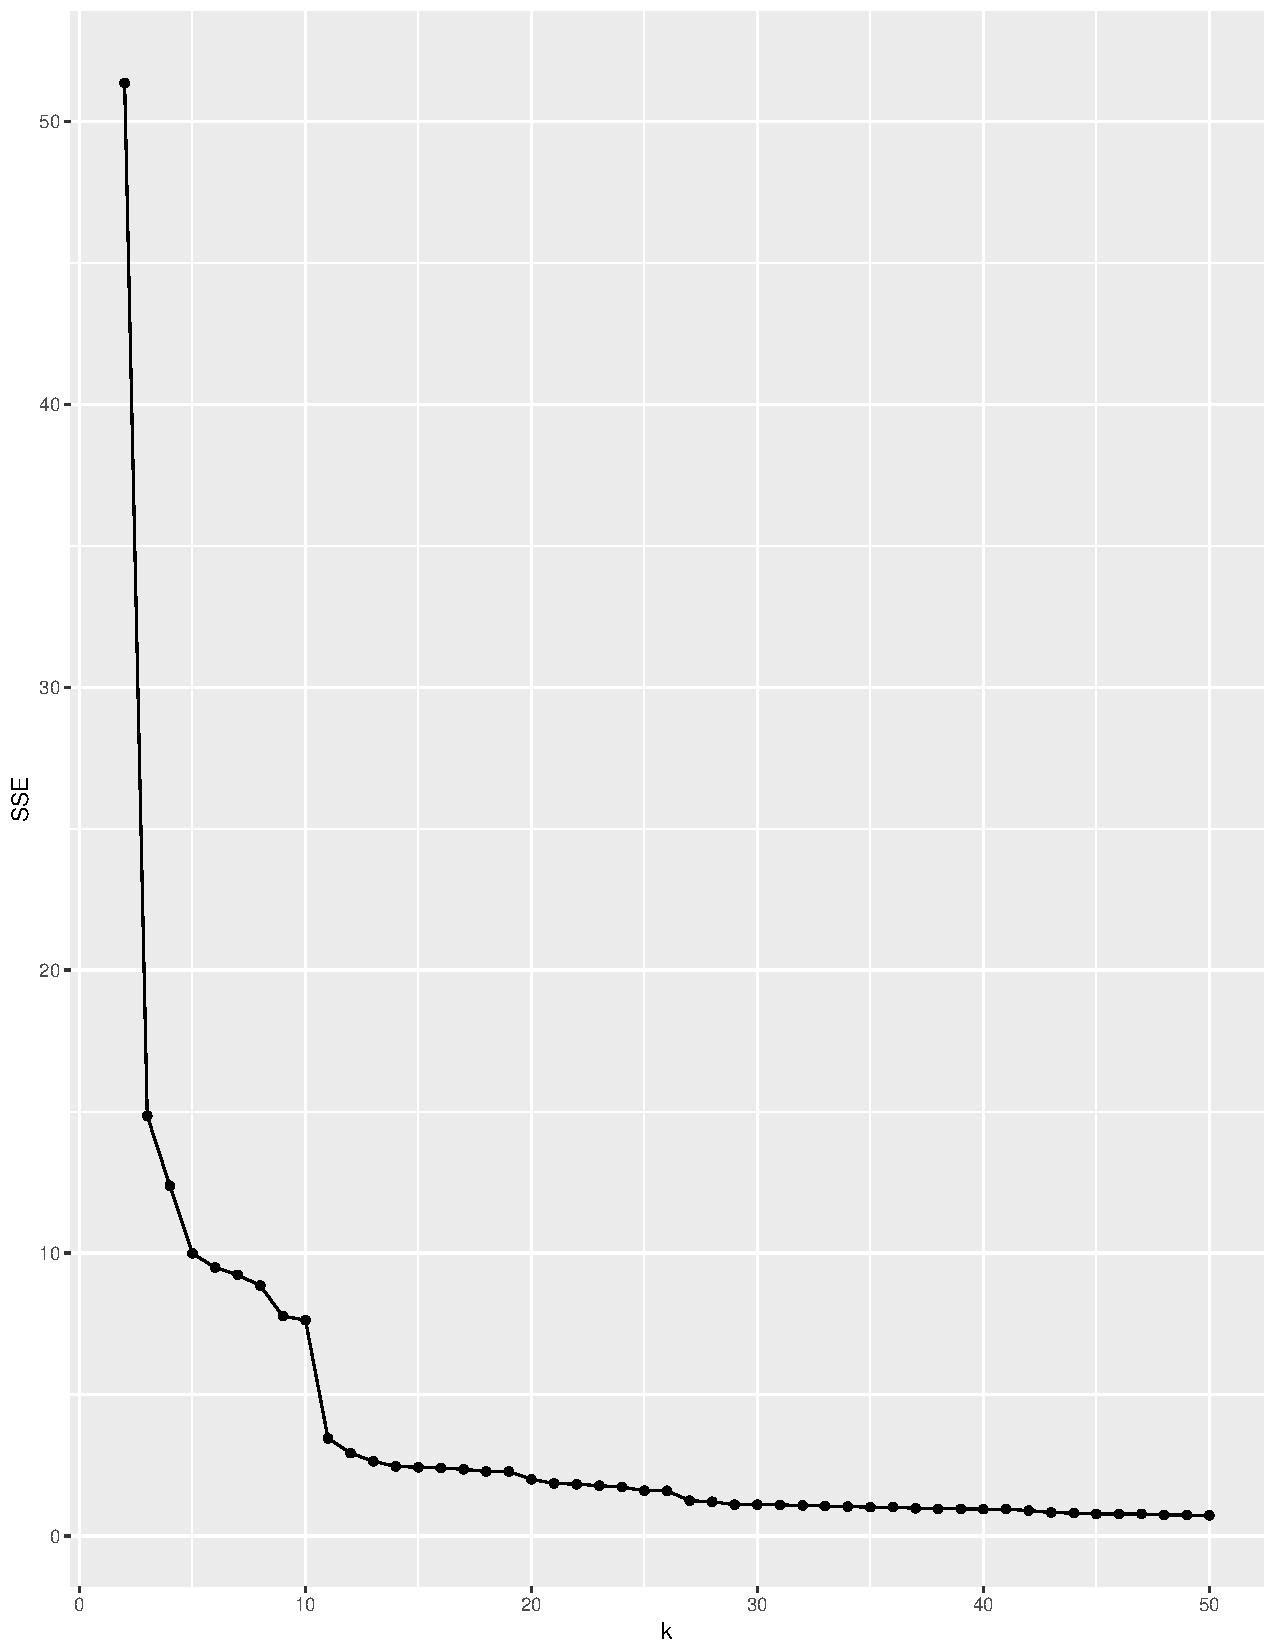
\includegraphics[width = 0.45\textwidth]{../img/k-sse-crediti-totali-arc-prg.pdf}
      \caption{Dependency update}
      \end{center}
    \end{figure}
\end{frame}

\begin{frame}{Example}
  \begin{figure}[bt]
    \begin{center}
    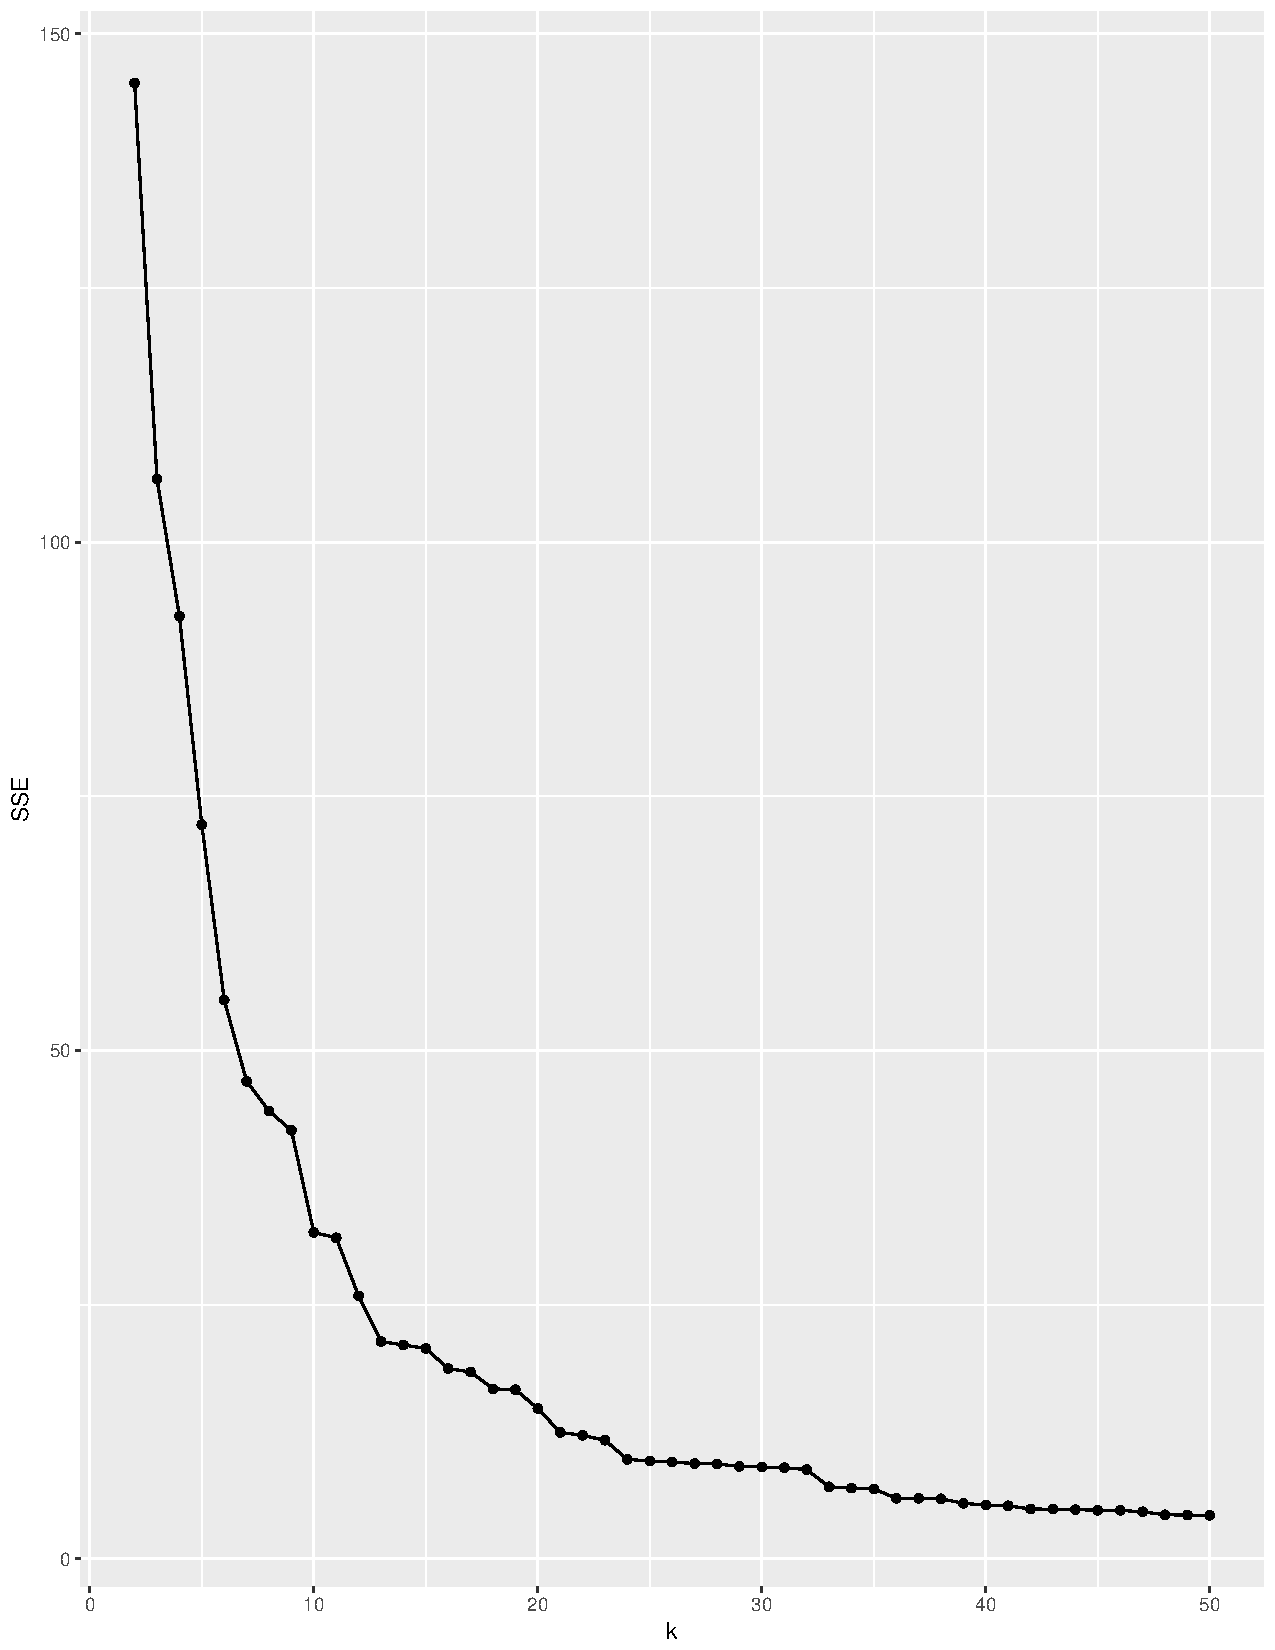
\includegraphics[width = 0.45\textwidth]{../img/k-sse-asd-arc-prg-an1-mdl.pdf}
    \caption{Dependency update}
    \end{center}
  \end{figure}
\end{frame}

\begin{frame}{Example}
    \begin{figure}[bt]
      \begin{center}
      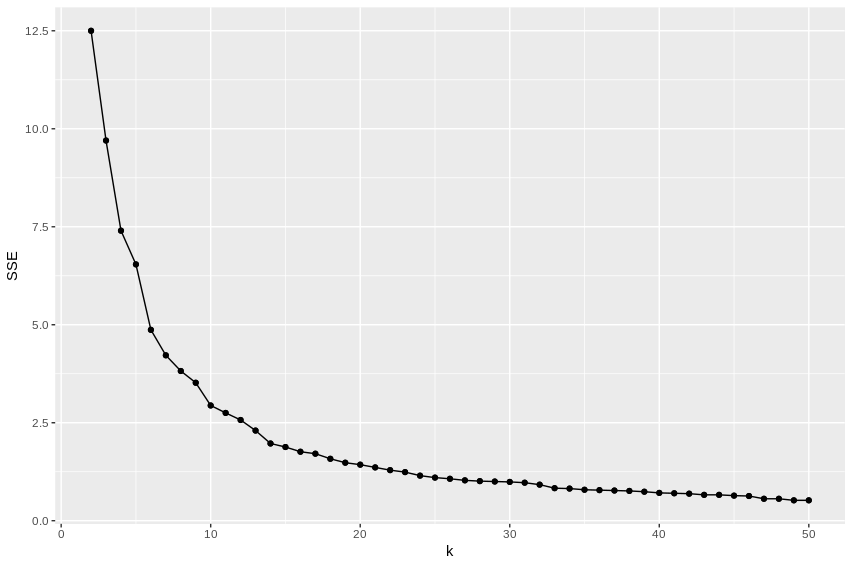
\includegraphics[width = 0.45\textwidth]{../img/k-sse-voto_medio-test.png}
      \caption{Dependency update}
      \end{center}
    \end{figure}
\end{frame}

\begin{frame}{Selezione \texttt{Eps} fissato \texttt{MinPts} in DBSCAN} 
    Viene effettuata tramite la seguente procedura
    \begin{itemize}
      \item Ordino i punti rispetto alla loro distanza dal loro $k$-esimo punto più vicino
      item pongo \texttt{MinPts}=$k$
      \item Determino un grafico con indici punti ordinati e distanze dal $k$-esimo più vicino 
      \item Selezione come valore di \texttt{Eps} quello per cui c'è un picco.
    \end{itemize} 
\end{frame}

\begin{frame}{Valutazione} 
    La valutazione dei clustering ottenuti con K-means e DBSCAN è stata fatta con la seguente procedura
    \begin{itemize}
      \item Calcolo matrice distanze tra i punti
      \item Calcolo matrice di incidenza dei cluster
      \item "Serializzazione" e calcolo della correlazione
    \end{itemize} 
    successivamente è possibile valutare e confrontare i risultati ottenuti dai clustering ottenuti
    con il K-means con i diversi valori di $k$ e con il DBSCAN.
\end{frame}

\begin{frame}[fragile]{SQL}
\begin{lstlisting}[style = R]
# Matrice di incidenza
matriceIncidenza <- function(data){
  nr = nrow(data)
  nc = ncol(data)
  C = matrix(nrow = nr, ncol = nr)
  for(i in 1:nr){
    for(j in 1:nr){
      if(data[i,nc] == data[j,nc])
        C[i,j] = 1
      else
        C[i,j] = 0
    }
  }
return(C)
\end{lstlisting}
\end{frame}

\begin{frame}[fragile]{SQL}
\begin{lstlisting}[style = R]
# matrice distanza
matriceDistanza <- function(data){
  return(as.matrix(dist(data[,1:(ncol(data)-1)],method = 'euclidean',diag = TRUE,upper = TRUE)))
}

calcoloCorrelazione <- function(data){
  MI <- matriceIncidenza(data)
  D <- matriceDistanza(data)
  mi = as.vector(t(MI))
  d = as.vector(t(D))
  
  return(cor(mi,d,method="pearson"))
}

calcoloCorrelazione(crediti_totali_prg_arc_clustered)
\end{lstlisting}
\end{frame}

\end{document}